\documentclass{beamer}
\usepackage[utf8]{inputenc}

\usetheme{Madrid}
\usecolortheme{default}
\usepackage{amsmath,amssymb,amsfonts,amsthm}
\usepackage{txfonts}
\usepackage{tkz-euclide}
\usepackage{listings}
\usepackage{adjustbox}
\usepackage{array}
\usepackage{tabularx}
\usepackage{gvv}
\usepackage{lmodern}
\usepackage{circuitikz}
\usepackage{tikz}
\usepackage{graphicx}

\setbeamertemplate{page number in head/foot}[totalframenumber]

\usepackage{tcolorbox}
\tcbuselibrary{minted,breakable,xparse,skins}



\definecolor{bg}{gray}{0.95}
\DeclareTCBListing{mintedbox}{O{}m!O{}}{%
  breakable=true,
  listing engine=minted,
  listing only,
  minted language=#2,
  minted style=default,
  minted options={%
    linenos,
    gobble=0,
    breaklines=true,
    breakafter=,,
    fontsize=\small,
    numbersep=8pt,
    #1},
  boxsep=0pt,
  left skip=0pt,
  right skip=0pt,
  left=25pt,
  right=0pt,
  top=3pt,
  bottom=3pt,
  arc=5pt,
  leftrule=0pt,
  rightrule=0pt,
  bottomrule=2pt,

  colback=bg,
  colframe=orange!70,
  enhanced,
  overlay={%
    \begin{tcbclipinterior}
    \fill[orange!20!white] (frame.south west) rectangle ([xshift=20pt]frame.north west);
    \end{tcbclipinterior}},
  #3,
}
\lstset{
    language=C,
    basicstyle=\ttfamily\small,
    keywordstyle=\color{blue},
    stringstyle=\color{orange},
    commentstyle=\color{green!60!black},
    numbers=left,
    numberstyle=\tiny\color{gray},
    breaklines=true,
    showstringspaces=false,
}
%------------------------------------------------------------
%This block of code defines the information to appear in the
%Title page
\title %optional
{2.10.19}
\date{\today}
%\subtitle{A short story}

\author % (optional)
{Shivam Sawarkar \\ AI25BTECH11031}


\begin{document}
\frame{\titlepage}

\begin{frame}{Quesiton}
     For three vectors $\Vec{u},\Vec{v},\vec{w}$ which of the following expression is not equal to any of the
 remaining three?
 \begin{enumerate}[a]
     \item $\vec{u}\cdot(\vec{v}\times\vec{w})$
     \item $\vec{v}\cdot(\vec{u}\times\vec{w})$
     \item $(\vec{v}\times\vec{w})\cdot\vec{u}$
     \item $(\vec{u}\times\vec{v})\cdot\vec{w}$
 \end{enumerate}
\end{frame}

\begin{frame}{Solution}
    As we know that dot product is cumulative so, $(1)$ and $(2)$ are equal \\
 That is,
\begin{align}
     \vec{u}^\top(\vec{v}\times\vec{w}) = (\vec{v}\times\vec{w})^\top\vec{u}
\end{align}

We prove
\begin{align}
\vec{u}^\top(\vec{v}\times\vec{w})=(\vec{u}\times\vec{v})^\top\vec{w}
\end{align}
\end{frame}

\begin{frame}{Solution}
    using the cross-product (skew-)matrix.

Define, for \(\vec{a}=(a_1,a_2,a_3)^T\),
\begin{align}
S(\vec{a})=\myvec{
0 & -a_3 & a_2\\
a_3 & 0 & -a_1\\
-a_2 & a_1 & 0
}
\end{align}

which satisfies $(\vec{a})\vec{b}=\vec{a}\times\vec{b}$  for all $\vec{b}\in\mathbb{R}^3$.
\end{frame}

\begin{frame}{Solution}
    \begin{align}
\vec{u}^\top(\vec{v}\times\vec{w})
&= \vec{u}^T\big(S(\vec{v})\vec{w}\big)
\quad\text{(since }S(\vec{v})\vec{w}=\vec{v}\times\vec{w}\text{)}\\ 
&= \big(\vec{u}^T S(\vec{v})\big)\vec{w} \\ 
&= \big(S(\vec{v})^T\vec{u}\big)^T\vec{w}
\quad\text{(transpose identity: }(A^T x)^T = x^T A\text{)}\\ 
&= \big(-S(\vec{v})\vec{u}\big)^T\vec{w}
\quad\text{(since }S(\vec{v})^T=-S(\vec{v})\text{)}\\ 
&= \big(\vec{u}\times\vec{v}\big)^T\vec{w}
\quad\text{(because }-S(\vec{v})\vec{u} = -(\vec{v}\times\vec{u}) = \vec{u}\times\vec{v})
\end{align}

Thus
\begin{align}
\vec{u}^\top(\vec{v}\times\vec{w}) = (\vec{u}\times\vec{v})^\top\vec{w}
\end{align}

This shows that (a), (c) and (d) are equal \\ 
\end{frame}

\begin{frame}{Example}
    Let
\begin{align}
\vec{u}=\myvec{1 \\ -1 \\ 1}, \quad \vec{v}=\myvec{0 \\ 1 \\ 2}, \quad \vec{w}=\myvec{1 \\ 0 \\ -1}.
\end{align}

Case 1: $\vec{u} ^\top (\vec{v} \times \vec{w})$

\begin{align}
\vec{v} \times \vec{w} =
\myvec{
v_{23} & w_{23} \\
v_{31} & w_{31} \\
v_{12} & w_{12}
}
=
\myvec{
v_2 w_3 - v_3 w_2 \\
v_3 w_1 - v_1 w_3 \\
v_1 w_2 - v_2 w_1
}
=
\myvec{
1 \times (-1) - 2 \times 0 \\
2 \times 1 - 0 \times (-1) \\
0 \times 0 - 1 \times 1
}
\end{align}


So
\begin{align}
\vec{v}\times \vec{w} = \myvec{-1 \\ 2 \\ -1}
\end{align}
\end{frame}

\begin{frame}{Examlpe}
Now compute the dot product:
\begin{align}
\vec{u} ^\top (\vec{v}\times \vec{w}) &= \myvec{1 & -1 & 1}\myvec{-1 \\ 2 \\ -1} \\
&= (1)(-1) + (-1)(2) + (1)(-1) \\
&= -4
\end{align}

\begin{align}
\boxed{\vec{u}^\top(\vec{v}\times \vec{w}) = -4}
\end{align}
\end{frame}

\begin{frame}{Example}
    Case 2: $\vec{v} ^\top (\vec{u} \times \vec{w})$

Compute $\vec{u} \times \vec{w}$:
\begin{align}
\vec{u} \times \vec{w} =
\myvec{
u_{23} & w_{23} \\
u_{31} & w_{31} \\
u_{12} & w_{12}
}
=
\myvec{
u_2 w_3 - u_3 w_2 \\
u_3 w_1 - u_1 w_3 \\
u_1 w_2 - u_2 w_1
}
=
\myvec{
(-1) \times (-1) - 1 \times 0 \\
1 \times 1 - 1 \times (-1) \\
1 \times 0 - (-1) \times 1
}
\end{align}

So
\begin{align}
\vec{u}\times \vec{w} = \myvec{1 \\ 2 \\ 1}.
\end{align}

Now compute dot product:
\begin{align}
\vec{v}^\top(\vec{u}\times \vec{w}) &= \myvec{0 & 1 & 2}\myvec{1 \\ 2 \\ 1} \\ 
&= 4.
\end{align}
\end{frame}

\begin{frame}{Example}
    Case 3: $(\vec{v} \times \vec{w}) ^\top \vec{u}$

We already have
\begin{align}
\vec{v}\times \vec{w} = \myvec{-1 \\ 2 \\ -1}
\end{align}

Now compute:
\begin{align}
(\vec{v}\times \vec{w})^\top \vec{u} &= \myvec{-1 & 2 & -1}\myvec{1 \\ -1 \\ 1} \\
&= (-1)(1) + (2)(-1) + (-1)(1) \\
&= -4.
\end{align}

\begin{align}
\boxed{(\vec{v}\times \vec{w})^\top \vec{u} = -4}
\end{align}
\end{frame}

\begin{frame}{Example}
    Case 4: $(\vec{u} \times \vec{v})^\top \vec{w}$

Compute $\vec{u} \times \vec{v}$:
\begin{align}
\vec{u} \times \vec{v} =
\myvec{
u_{23} & v_{23} \\
u_{31} & v_{31} \\
u_{12} & v_{12}
}
=
\myvec{
u_2 v_3 - u_3 v_2 \\
u_3 v_1 - u_1 v_3 \\
u_1 v_2 - u_2 v_1
}
=
\myvec{
(-1) \times 2 - 1 \times 1 \\
1 \times 0 - (-1) \times 2 \\
1 \times 1 - (-1) \times 0
}
\end{align}

So
\begin{align}
\vec{u}\times \vec{v} =\myvec{-3 \\ -2 \\ 1}
\end{align}

Now compute:
\begin{align}
(\vec{u}\times \vec{v})^\top \vec{w} &= \myvec{-3 & -2 & 1}\myvec{1 \\ 0 \\ -1} \\
&= (-3)(1) + (-2)(0) + (1)(-1) \\
&= -4.
\end{align}
\end{frame}

\begin{frame}{Example}
    Final Results
\begin{align}
\vec{u}^\top(\vec{v}\times \vec{w})=-4, \\ 
\vec{v}^\top(\vec{u}\times \vec{w})=4, \\ 
(\vec{v}\times \vec{w})^\top \vec{u}=-4, \\ 
(\vec{u}\times \vec{v})^\top \vec{w}=-4
\end{align}

Thus (a), (c) and (d) are same
\end{frame}

\begin{frame}{Plot}

    \begin{figure}
        \centering
        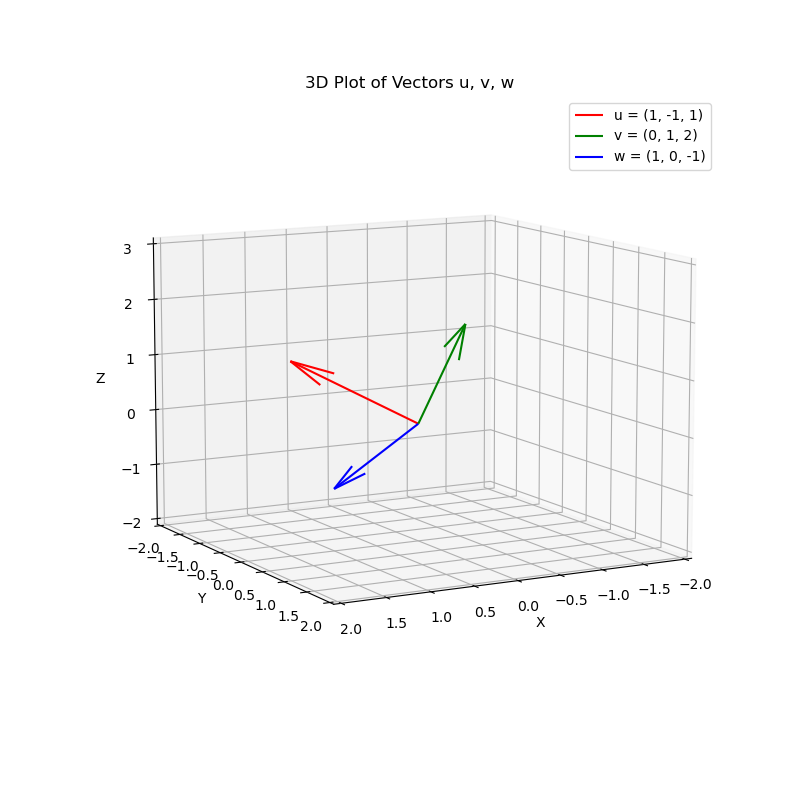
\includegraphics[width=0.5\linewidth]{figs/plot5.png}
        \caption{}
        \label{fig:placeholder}
    \end{figure}
\end{frame}

\begin{frame}[fragile]{C Code}
    \begin{verbatim}
#ifndef VECTOROPS_H
#define VECTOROPS_H

// Function to compute cross product of two vectors
void cross(int a[3], int b[3], int result[3]) {
    result[0] = a[1]*b[2] - a[2]*b[1];
    result[1] = a[2]*b[0] - a[0]*b[2];
    result[2] = a[0]*b[1] - a[1]*b[0];
}

// Function to compute dot product of two vectors
int dot(int a[3], int b[3]) {
    return a[0]*b[0] + a[1]*b[1] + a[2]*b[2];
}

#endif
    \end{verbatim}
\end{frame}

\begin{frame}[fragile]{C Code}
    \begin{verbatim}
#include <stdio.h>
#include "vectorops.h"

int main() {
    int u[3], v[3], w[3];
    int temp[3];
    int A, B, C, D;

    // Input vectors
    printf("Enter vector u (x y z): ");
    scanf("%d %d %d", &u[0], &u[1], &u[2]);
    printf("Enter vector v (x y z): ");
    scanf("%d %d %d", &v[0], &v[1], &v[2]);
    printf("Enter vector w (x y z): ");
    scanf("%d %d %d", &w[0], &w[1], &w[2]);
    \end{verbatim}
\end{frame}

\begin{frame}[fragile]{C Code}
    \begin{verbatim}
    cross(v, w, temp);
    A = dot(u, temp);
    cross(u, w, temp);
    B = dot(v, temp);
    cross(v, w, temp);
    C = dot(temp, u);
    cross(u, v, temp);
    D = dot(temp, w);
    printf("\nResults:\n");
    printf("A = u · (v × w) = %d\n", A);
    printf("B = v · (u × w) = %d\n", B);
    printf("C = (v × w) · u = %d\n", C);
    printf("D = (u × v) · w = %d\n", D);
    printf("B is different");
    return 0;
}
    \end{verbatim}
\end{frame}

\begin{frame}[fragile]{Python + C Code}
    \begin{verbatim}
import ctypes
import numpy as np
import matplotlib.pyplot as plt

# Load shared library
lib = ctypes.CDLL("./libvectorops.so")

# Define function signatures
lib.dot.argtypes = [ctypes.POINTER(ctypes.c_int), ctypes.POINTER(ctypes.c_int)]
lib.dot.restype = ctypes.c_int

lib.cross.argtypes = [ctypes.POINTER(ctypes.c_int), ctypes.POINTER(ctypes.c_int), ctypes.POINTER(ctypes.c_int)]
lib.cross.restype = None
    \end{verbatim}
\end{frame}

\begin{frame}[fragile]{Python + C Code}
    \begin{verbatim}
def dot(a, b):
    a_arr = (ctypes.c_int * 3)(*a)
    b_arr = (ctypes.c_int * 3)(*b)
    return lib.dot(a_arr, b_arr)
def cross(a, b):
    a_arr = (ctypes.c_int * 3)(*a)
    b_arr = (ctypes.c_int * 3)(*b)
    result = (ctypes.c_int * 3)()
    lib.cross(a_arr, b_arr, result)
    return [result[0], result[1], result[2]]
def compute(u, v, w):
    A = dot(u, cross(v, w))      # u · (v × w)
    B = dot(v, cross(u, w))      # v · (u × w)
    C = dot(cross(v, w), u)      # (v × w) · u
    D = dot(cross(u, v), w)      # (u × v) · w
    return A, B, C, D
    \end{verbatim}
\end{frame}

\begin{frame}[fragile]{Python + C Code}
    \begin{verbatim}
    u = list(map(int, input("Enter vector u (x y z): ").split()))
    v = list(map(int, input("Enter vector v (x y z): ").split()))
    w = list(map(int, input("Enter vector w (x y z): ").split()))

    A, B, C, D = compute(u, v, w)

    print("\nResults:")
    print(f"A = u · (v × w) = {A}")
    print(f"B = v · (u × w) = {B}")
    print(f"C = (v × w) · u = {C}")
    print(f"D = (u × v) · w = {D}")
    print("\n=> Expression B is different.")
    \end{verbatim}
\end{frame}

\begin{frame}[fragile]{Python Code}
    \begin{verbatim}
def dot(a, b):
    return a[0]*b[0] + a[1]*b[1] + a[2]*b[2]

def cross(a, b):
    return [
        a[1]*b[2] - a[2]*b[1],
        a[2]*b[0] - a[0]*b[2],
        a[0]*b[1] - a[1]*b[0]
    ]
    \end{verbatim}
\end{frame}

\begin{frame}[fragile]{Python Code}
    \begin{verbatim}
def main():
    u = list(map(int, input("Enter vector u (x y z): ").split()))
    v = list(map(int, input("Enter vector v (x y z): ").split()))
    w = list(map(int, input("Enter vector w (x y z): ").split()))
    A = dot(u, cross(v, w))
    B = dot(v, cross(u, w)
    C = dot(cross(v, w), u)
    D = dot(cross(u, v), w)
    print("\nResults:")
    print(f"A = u · (v × w) = {A}")
    print(f"B = v · (u × w) = {B}")
    print(f"C = (v × w) · u = {C}")
    print(f"D = (u × v) · w = {D}")
    print("\n=> Expression B is different.")
    \end{verbatim}
\end{frame}



\end{document}